\section{ROS}
\noindent Robotický operačný systém (\acrlong{ROS}) je súbor voľne dostupných softvérových knižníc a nástrojov, ktoré nám vytvárajú
vhodné podmienky na písanie aplikácií pre mnohé druhy robotov. ROS má dve verzie. Vo všeobecnosti sa stretneme s tým, že pod názvom
ROS1 alebo ROS sa myslí ROS verzie 1. Pod názvom ROS2 sa myslí ROS verzie 2. Aby nenastali nejasnosti budeme v tomto dokumente
označovať ROS verzie 1 ako ROS1 a ROS verzie 2 ako ROS2 V prípade, keď budme hovoriť o spoločných vlastnostiach a funkcionalitách,
ROS1 a ROS2 budeme označovať dokopy ako ROS.

\subsection{ROS}

\noindent Komunikácia v ROSe je zabezpečená cez IPC (\acrlong{IPC}), TCP/IP UDP/IP komunikáciou pomocou troch zakladacích metód:
\textbf{topiky} (Topics), \textbf{služby} (Service) a \textbf{akcie} (Actions)

\subsubsection{Topiky}

\textbf {Topiky} (IPC) sú najjednoduchší spôsob komunikácie. Vieme si ich prirovnať k UDP/IP protokolu. Definujeme si jedného poskytovateľa (publisher)
a jedného príjemcu (subscriber). Medzi týmito dvoma účastníkmi sa následne posielajú správy (messages), ktoré sme si dopredu definovali.

\begin{figure}[h]
	\centering
	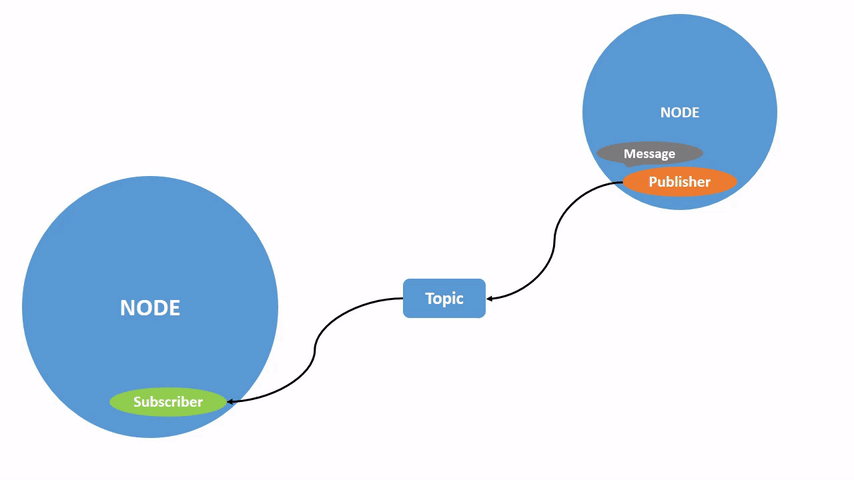
\includegraphics[width=8cm]{img/topicsExplanation.png}
	\caption{Vizualizacia topicu v ROSe \cite{RosDoc}}
	\label{fig:topics}
\end{figure}

\subsubsection{Služby}

\textbf {Služby} (TCP/IP) nám poskytujú rovnaký spôsob komunikácie ako topiky, až na to, že sa správy medzi servisom a klientom posielajú
cez LAN (\acrlong{LAN}). Služby sa využívajú pri komunikácii medzi viacerými zariadeniami.

\begin{figure}[h]
	\centering
	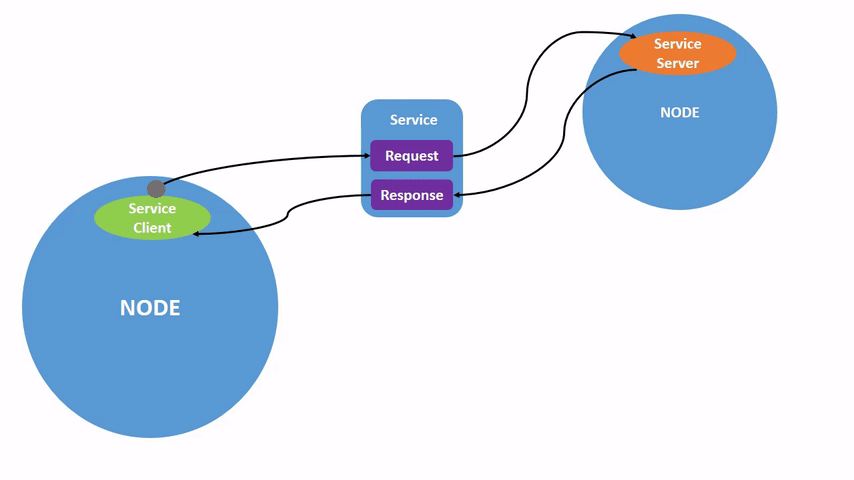
\includegraphics[width=8cm]{img/serviceExplanation.png}
	\caption{Vizualizácia služby v ROSe \cite{RosDoc}}
	\label{fig:service}
\end{figure}

\subsubsection{Akcie}

\label{s_action}
\textbf {Akcie} (TCP/IP) sú najzložitejším spôsobom komunikácie. Tento spôsob bol pridaný do ROS1 až neskor. V druhej verzii ROSu je tento
typ komunikácie medzi troma základnými. Sú založené na službách a máju 3 stavy. Najprv pošle klient serveru akú akciu má vykonať, server mu potvrdí,
že túto požiadavku dostal. Server začne následne vykonávať danú akciu a posielať klientovi priebežné správy o priebehu. Keď server skončí pošle
klientovi výsledok akcie a klient mu obratom potvrdí obdržanie výsledku.

\begin{figure}[h]
	\centering
	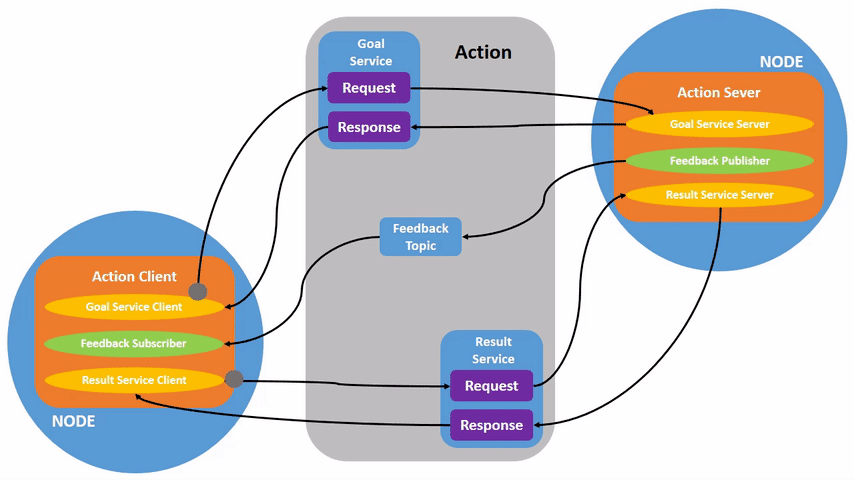
\includegraphics[width=8cm]{img/actionExplanation.png}
	\caption{Vizualizácia akcie v ROSe \cite{RosDoc}}
	\label{fig:action}
\end{figure}

\begin{figure}[!htbp]
	\centering
	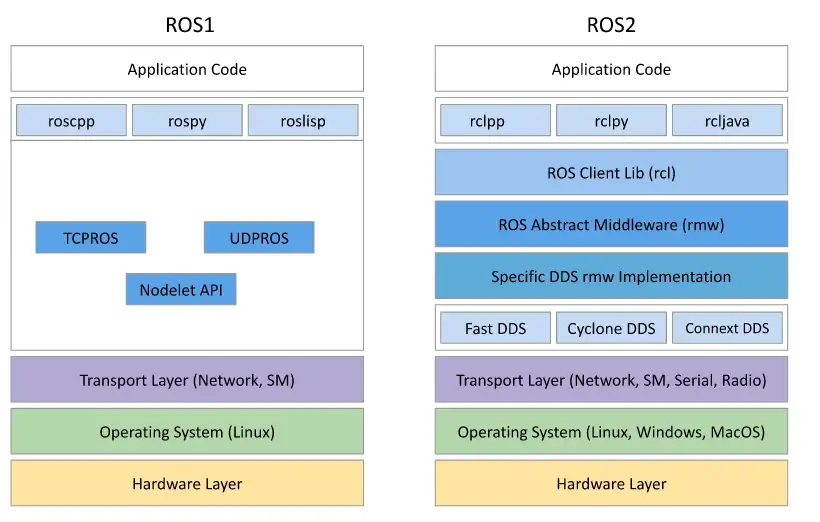
\includegraphics[width=15cm]{img/strukturaRos1Ros2.png}
	\caption{Porovnanie štruktúr ROS1 a ROS2 \cite{comparison}}
	\label{fig:struktury}
\end{figure}

\pagebreak

\subsection{ROS1}

\noindent ROS bol prvýkrát vydaný v roku 2007. Ide o softvér, ktorý sa začal vyvíjať so zámerom zjednodušiť programovanie a ovládanie robotov. Od doby,
kedy vznikol prešiel mnohými verziami a úpravami. Jeho neoddeliteľnou súčasťou sú štrukturalizovanie programu do uzlov (nodov), komunikácia medzi uzlami,
podpora viacerých programovacích jazykov ako sú C, C++ alebo Python a vytváranie balíčkov dostupných širokej verejnosti.

Štrukturalizovanie základov ROS1 je spravené monoliticky čo najstabilnejším spôsobom. Na počiatku programu musíme spustiť hlavný program (roscore),
ktorý zabezpečuje vytváranie jednotlivých uzlov. Komunikácia medzi uzlami je zabezpečená prostredníctvom prepojenia uzlov cez LAN/WLAN alebo IPC komunikaciu.
Uzly môžu byť spustené aj na iných zariadeniach. Roscore ďalej poskytuje parametre jednotlivým uzlom z parametrového servera. Jeho najväčšou úlohou je zabezpečenie
komunikácie uzlov v programe. Nezáleží na tom, či sú uzly na jednom alebo viacerých zariadeniach.

\pagebreak

Aj napriek mnohým výhodám má ROS aj nedostatky, ktoré sa ťahajú už od jeho počiatkov. Sú to napríklad:
\begin{itemize}
	\item Nepostačujúca distribuovanosť systému. Ak prestane fungovať roscore, prestane ísť celý program,
	\item ROS1 je písaný v starom štandarde a to vnáša do programu technologický dlh a bezpečnostné riziká,
	\item Kvalita komunikácie sa nedá ovplyvniť
\end{itemize}

Kvôli takýmto problémom sa začala vyvíjať nová verzia ROSu, ROS2. V roku 2025 sa skončí podpora poslednej distribúcie ROS1 menom Noetic.
Preto je odporúčané začínať nové projekty v ROS2.

\subsection{ROS2}

Ako už bolo spomenuté zámerom vývoja ROS2 je zlepšenie funkcionality a bezpečnosti systému. ROS2 nie je spätne kompatibilný.
Podstata toho, ako sú zoskupované uzly a ako spolu komunikujú je diametrálne odlišná od ROS1. Z tohto dôvodu bol vyvinutý takzvaný rosbridge,
ktorý zabezpečuje kompatibilitu medzi verziami. Nie je to ale trvalé riešenie. Odporúčané je nástroj využívať a počas toho prepisovať kód
z verzie 1 do verzie 2. Komunikácia prebieha \newline v ROS2 rovnakým spôsobom ako v ROS1. Pomocou topikov, služieb a akcií.

Táto podobnosť končí na najvyššej vrstve. Ako sme videli na Obr.~\ref{fig:struktury}. Štruktúra ROS2 je rozdelená do viacerých vrstiev.
Najdôležitejšie je pre nás vedieť, že komunikácia je spracovávaná modelom DDS (Služba distribúcie údajov) z anglického (\acrlong{DDS}). Tento model zlepšuje výkon, stabilitu
a bezpečnosť modelu oproti ROS1. Je založený na TCP/UDP protokole. Z obrázku vyčítame aj lepšie rozloženie modulov. To zabezpečuje jednoduchšie
prispôsobovanie systému pre nové funkcionality. Podpora operačných systémov sa v ROS2 rozšírila aj o Windows, Mac OS či operačné systémy reálneho času.
Operačne systémy nie sú jediné rozšírenie ohľadom kompatibility. S ROS2 je možné programovať už aj v Jave či Matlabe.
Tvorcovia mysleli aj na programátorov a pridali rozšírené možnosti testovania, debugovania či nasadzovania programu do reálneho využitia.

ROS2 ma necentralizovanú štruktúru, a preto pri spúšťaní programov už nie je potrebné mať spustený roscore. Ak teda spadne
jeden proces druhé budú fungovať naďalej. V ROS1 sme vedeli ovplyvniť počet uchovaných správ pokým nepretiekol zásobník, ktorý ich uchovával na neskoršie použitie.
V ROS2 vieme zmeniť kvalitu komunikácie. Vieme si zadefinovať, či by sme radšej stratili niektoré správy, ale dostali by sme všetky rýchlo. Alebo aby sa zabezpečilo,
že dostaneme všetky správy, ktoré boli vyslané, aj keby to trvalo dlhšie. Dokonca si vieme zadefinovať maximálny čas, ktorý budeme čakať na ďalšiu správu.

Pri všetkých týchto zlepšeniach nemôžeme zabudnúť aj nasledovný nedostatok. Keďže ROS2 je mladší ako ROS1 nájdeme k nemu menej dokumentácie.
Pridaním veľkého počtu funkcionalít začal vznikať problém pre začiatočníkov s porozumením niektorých kódov. Avšak tento problém je nedostatkom,
ktorý časom zanikne. V čase písania tejto prace pribudli na stránke dokumentácie 2 strany popisujúce pokročilejšie Funkcionality druhej verzie ROSu.

\subsection{Rozdiely}

Čo je určite dobrou správou pre všetkých programátorov, ktorí robili v prvej verzii a sú zvyknutí na jej štandardy a funkcionalitu sa nemajú čoho obávať.
Prechod z ROS1 na ROS2 je dosť priamočiary. Čo sa zmenilo je spôsob písania kódu, ale koncepty funkcionality ostali všetky rovnaké. V tejto sekcii nebudeme
písať konkrétne kódy, budeme len opisovať čo je podobné a čo zasa rozdielne medzi verziami spomínaného systému. Keďže celý projekt bol písaný v programovacom
jazyku C++ tak sa aj tieto zmeny budu týkať hlavne C++.

\subsubsection{Štandard jazyka}

	Pokým ROS1 bola písaná v štandarde C++98 tak ROS2 je už písaná v novom štandarde. To zahŕňa inicializovanie templatov a ich použivanie. Definície
	a deklarácie templatov sú na knihu samú o sebe, preto do detailov nebudeme zachádzať. Stačí nám vedieť, ako ich inicializovať. V prvej verzii
	sme definovali publishera (publikovateľa) všeobecného a definovali sme mu cez aký topic má posielať správy. V druhej verzii naväzujeme publishera
	na špecifický tip správy akú posielame. Nemôže sa teda stať, že takýto program by sme skompilovali a následne keď ho spustíme tak by spadol.

\subsubsection{Inicializácia nody}

	Tak isto ako v prvej verzii aj v druhej verzii musíme definovať nodu. Rozdiel je v tom, že prvá verzia obsahovala NodeHandle a druha verzia obsahuje priamo Node.
	V druhej verzii je zaužívaným štandardom tuto nodu precediť a použiť polymorfizmus pri objekte, ktorý musí existovať počas celej doby vykonávania programu. Pri
	prvej verzii tomu tak nebolo. Museli sme vytvoriť už spomenutý NodeHandle. Ten sa nemusel využiť ako base trieda a nemusel ani existovať počas celého behu programu.

\subsubsection{Komunikácia}

	DDS (Služba distribúcie údajov) je stredný protokol používaný v ROS2 na komunikáciu medzi uzlami. Je to systém správ
	publikovania (publish) / odoberania (subscribe), ktorý umožňuje uzlom komunikovať medzi sebou bez toho, aby poznali identitu ostatných uzlov. DDS je
	štandardný protokol, ktorý sa okrem ROS2 používa vo viacerých odvetviach. \cite{chatgpt} Druh komunikácie je v ROS2 rozšírený ešte o akcie \ref{s_action}.

\subsubsection{Vlákna}

	Prvá verzia ROSu je založená na jedno vláknovom, synchrónnom komunikačnom modeli, zatiaľ čo ROS2 je založený na viac vláknovom, asynchrónnom
	komunikačnom modeli. Táto zmena znateľne zrýchľuje program, ale prináša väčšiu komplexnosť do programu.

\subsubsection{Kompilácia}

	Zmenou verzii sa zmenil aj spôsob kompilácie programu. ROS1 bol skompilovaný pomocou \texttt{catkin} build systému. Catkin je založený na programe
	\texttt{cmake}. Jeho nastavenie dependencií je konfigurované pomocou súboru \texttt{package.xml} . ROS2 prešiel na viac nastaviteľný systém \texttt{Colcon}.
	Tento systém je na rozdiel od catkinu založený na Pythone a jeho dependencie sa nastavujú pomocou \texttt{setup.py} súboru. V prípade colconu si môžeme definovať
	spôsob kompilácie t.j. môžeme nastaviť, ako sa budú spracovávať dependencie. Jednou s najviac používaných možností je \texttt{ament\_cmake}. Je založený
	na cmaku a spolupracuje s colconom. Medze ament\_cmake je založený na cmaku vieme mu definovať dependencie pomocou xml súboru ako v ROS1. Je to jeden zo spôsobov,
	ako zmenšiť rozdiel medzi ROS1 a ROS2.

\section{Robot}

Robot, s ktorým sme pracovali bol výsledkom tímového projektu viacerých študentov \newline z roku 2019. Pri vysvetľovaní a opisovaní robota sa budeme odvolávať
na dokumenty, stránky a kód, ktorý napísali. Všetky tieto údaje si sprístupnené na mobilnom robote v záložke
\newline \texttt{\$(HOME)/Desktop/Blackmetal}~\cite{timovyProjekt}.

Robot je v tvare kvádra. Jeho šírka je 60cm a je vyzdvihnutý nad zem o 1.5cm. Nachádza sa na kolesách o polomere 8cm. Jeho kostra, až na oceľové pláty, ktoré držia robot,
je spravená z hliníku. Konkrétne z hliníkových tyčí, ktoré sú pospájané plexisklovými plátmi. 

\begin{figure}[!htbp]
	\begin{center}
		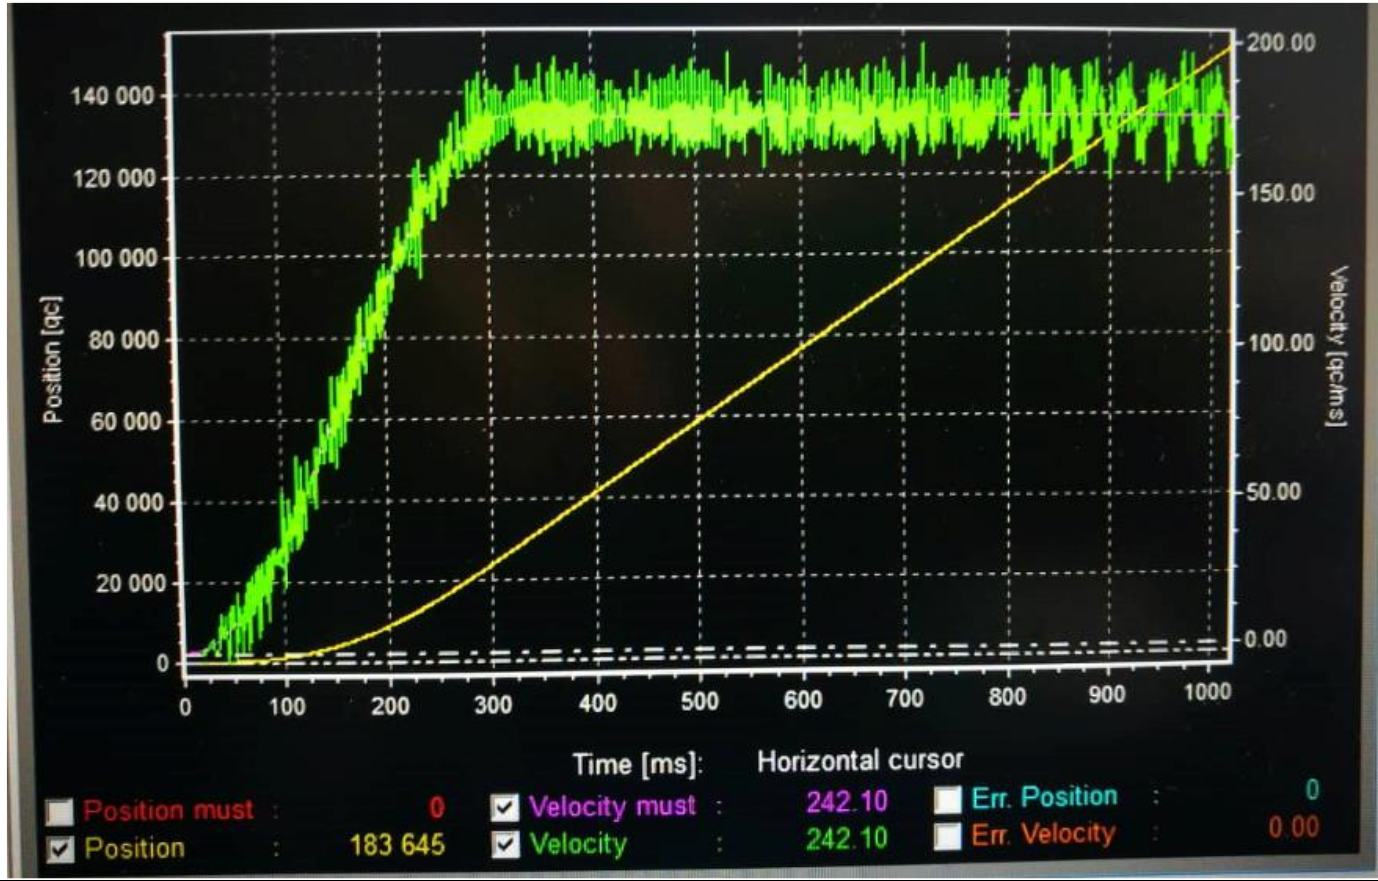
\includegraphics[width=0.95\textwidth]{img/robotSpeedChar.png}
	\end{center}
	\caption{Prechodová charakteristika rýchlosti kolies \cite{timovyProjekt}. }
	\label{fig:prechChar}
\end{figure}

\subsection{Lorem Ipsum}
Tento text bol prevzaty zo stranky \url{www.lipsum.com} \cite{lipsum}, preto ho treba riadne odcitovat.

Lorem Ipsum is simply dummy text of the printing and typesetting industry. Lorem Ipsum has been the industry's standard dummy text ever since the 1500s, when an unknown printer took a galley of type and scrambled it to make a type specimen book. It has survived not only five centuries, but also the leap into electronic typesetting, remaining essentially unchanged. It was popularised in the 1960s with the release of Letraset sheets containing Lorem Ipsum passages, and more recently with desktop publishing software like Aldus PageMaker including versions of Lorem Ipsum \cite{lipsum}.

Why do we use it? It is a long established fact that a reader will be distracted by the readable content of a page when looking at its layout. The point of using Lorem Ipsum is that it has a more-or-less normal distribution of letters, as opposed to using 'Content here, content here', making it look like readable English \cite{lipsum}. Many desktop publishing packages and web page editors now use Lorem Ipsum as their default model text, and a search for 'lorem ipsum' will uncover many web sites still in their infancy. Various versions have evolved over the years, sometimes by accident, sometimes on purpose (injected humour and the like).

Where does it come from? Contrary to popular belief, Lorem Ipsum is not simply random text. It has roots in a piece of classical Latin literature from 45 BC, making it over 2000 years old. Richard McClintock, a Latin professor at Hampden-Sydney College in Virginia, looked up one of the more obscure Latin words, consectetur, from a Lorem Ipsum passage, and going through the cites of the word in classical literature, discovered the undoubtable source \cite{lipsum}. Lorem Ipsum comes from sections 1.10.32 and 1.10.33 of "de Finibus Bonorum et Malorum" (The Extremes of Good and Evil) by Cicero, written in 45 BC. This book is a treatise on the theory of ethics, very popular during the Renaissance. The first line of Lorem Ipsum, "Lorem ipsum dolor sit amet..", comes from a line in section 1.10.32 \cite{lipsum}.

\section{Recitácia}
Citujem všetky zdroje v \textbf{bibliography.bib}, \cite{t00, t01, t02, t03, kniha, kniha2, kniha3, small, big, cs, koll, kap, tug, knuth, zbornik, prispevok}. \newline Good luck.

\section{Rovnice}
Pytagorova veta je definovana vztahom:
\begin{equation}
	a^2 + b^2 = c^2
	\label{eq:pyth}
\end{equation}
Dosadenim \eqref{eq:pyth} do linearneho modelu
\begin{align}
	\dot{\mathbf{x}} &= \mathbf{A} \mathbf{x} + \mathbf{B} \mathbf{u} \\
	\mathbf{y} &= \mathbf{C} \mathbf{x} + \mathbf{D} \mathbf{u}
	\label{eq:model}
\end{align}
zistime, ze tento \LaTeX template funguje, dokonca mozeme vkladat aj inline rovnice $D = b^2 - 4ac$.

% \subsection{Podsekcia}
% \begin{equation}
%	 E = m c^2
%	 \label{eq:emc2}
% \end{equation}

\section{Možnosti anonymizácie}
\noindent Anonymizácia znamená zmena alebo úprava údajov tak, aby sa podľa nich nedala jednoznačne určiť osoba, ktorej tieto údaje patria \cite{t01}. Existuje niekoľko spôsobov, ktorými môžeme dosiahnuť rôznu úroveň anonymizácie na internete: od mazania cookies súborov po ukončení prehliadania webových stránok až po používanie operačných systémov, ktoré sú na anonymite založené; od bezplatných možností až po komerčné verzie.
\newline Nasleduje priblíženie niektorých možnosti anonymizácie.

\subsection{Súkromné prehliadanie}
\noindent Najpoužívanejšie internetové prehliadače súčasnosti majú v sebe zabudovanú funkcionalitu, ktorá dokáže čiastočne anonymizovať prístup na internet. Táto funkcionalita blokuje ukladanie navštívených stránok do histórie a nezaznamenáva súbory, ktoré sa stiahnu z~internetu. sw a hw sú skratky.

\begin{table}[!htbp]
\caption{Moduly a ich funkcie pri anonymizácii}
\label{modulyVlastnosti}
\begin{center}
\begin{tabular}{p{4cm}|c|c|c|c|c|c|c|c|c|c|c|c|c|c|c}
& \multicolumn{14}{c}%
	 {\textbf{Funkcia}}\\ \hline
&&&& & &\multicolumn{8}{c}%
	 {Modifikácia}\\
\textbf{Modul} &\begin{sideways} zobrazenie hlavičky \end{sideways} &\begin{sideways} blokovanie skriptov \end{sideways} &\begin{sideways} zmena IP \end{sideways} & \begin{sideways} zmena lokalizácie \end{sideways} & \begin{sideways} zmazanie/blokovanie cookies \end{sideways} & \begin{sideways} blokovanie trackerov \end{sideways}  & \begin{sideways} popis \end{sideways} & \begin{sideways}používateľský agent\end{sideways} & \begin{sideways} kódové označenie prehliadača \end{sideways} & \begin{sideways} názov prehliadača \end{sideways} & \begin{sideways} verzia prehliadača \end{sideways} & \begin{sideways} platforma \end{sideways} & \begin{sideways} výrobca prehliadača \end{sideways} & \begin{sideways} označenie výrobcu prehliadača \end{sideways} \\ \hline
User agent switcher & & & & & &  & X & X & X & X & X & X & X & X  \\ \hline
Ghostery &  && & & X & X &  &  & & & & & & \\  \hline
Better privacy && &  & & X &  &  &  & & & & & & \\  \hline
Anonymox &  && X & X & X &  & X & X & & & & & & \\  \hline
Modify headers & & &  &  & X &  &  & X &  &  &  & & &  \\  \hline
Request policy & & &  &  & & X  &  &  &  &  &  & & &   \\  \hline
Live HTTP headers & X& &  &  & &  &  &  &  &  &  & & &   \\  \hline
User agent awitcher for chrome & & &  &  & &  & X & X &  &  &  & & &   \\  \hline
Header hacker & & &  &  & &  & X & X & X & X & X & X & X & X	\\  \hline
Mod header & & &  &  & &  & X & X & X & X & X & X & X & X	\\  \hline
Script no & &X &  &  & &  &  &  &  &  &  &  &  &	 \\  \hline
No script & &X &  &  & &  &  &  &  &  &  &  &  &	 \\  \hline
Proxify it & & &X  & X & &  &  &  &  &  &  &  &  &	 \\  \hline
I'm not here & & &  & X & &  &  &  &  &  &  &  &  &	 \\  \hline
Get anonymous personal edition & &X &X &X &X&X &  &  &  &  &  &  &  &	 \\  \hline
Anonymous browsing toolbar & & & X & X & &  &  &  &  &  &  &  &  &	 \\  \hline
Easy hide your IP and surf anonymously & & & X & X& &  &  & X & X & X & X &  &  &	 \\  \hline
\end{tabular}
\end{center}
\end{table}

\subsection{Anonymná sieť}
\noindent Anonymná sieť je sieť serverov, medzi ktorými dáta prechádzajú šifrované. V anonymných sieťach dáta prechádzajú z počítača používateľa, odkiaľ bola požiadavka poslaná, cez viaceré proxy smerovače, z ktorých každý správu doplní o smerovanie a zašifruje vlastným kľúčom. Cesta od ...


\subsection{Funkcionalita}
\noindent  Rozšírenie tiež okrem splnenia špecifikácie malo pre prehľadnosť a overenie funkčnosti zobrazovať údaje, ktoré boli na server odoslané. Zoznam údajov odoslaných na server, sa mal ukladať do krátkodobej histórie, aby nemal používateľ k dispozícií len najnovšie údaje, ale aj údaje odoslané v nejakom časovom období. Nejaky listing z priloh \ref{lst:sublime}.

\subsubsection{Funkcionalita2}
\noindent Samozrejmosťou bolo nastavenie zapnutia rozšírenia pri štarte, prípadne interval zmeny odosielaných údajov.

\subsection{Vzhľad}
\noindent Dôležitou požiadavkou kladenou na rozšírenie bolo príjemné používateľské rozhranie. Z~tohto dôvodu malo rozšírenie obsahovať zoznam modifikovaných vlastností a tlačidlo pre prístup k nastaveniam rozšírenia v jednoduchej a praktickej forme. Predpokladaný vzhľad je zobrazený na obrázku č. \ref{vzhladobr}.
\begin{figure}[!htbp]
	\centering
	\includegraphics[width=8cm]{img/vzhlad.png}
	\caption{Predpokladaný vzhľad rozšírenia}
	\label{vzhladobr}
\end{figure}
\noindent Dôležitou požiadavkou kladenou na rozšírenie bolo príjemné používateľské rozhranie.\cite{t00} Z~tohto dôvodu malo rozšírenie obsahovať zoznam modifikovaných vlastností a tlačidlo pre prístup k nastaveniam rozšírenia v jednoduchej a praktickej forme. Predpokladaný vzhľad je zobrazený na obrázku č. \ref{vzhladobr}.

\begin{algorithm}
\scriptsize
\begin{algorithmic}
	\STATE <text>
	\IF{<condition>} \STATE {<text>} \ELSE \STATE{<text>} \ENDIF
	\IF{<condition>} \STATE {<text>} \ELSIF{<condition>} \STATE{<text>} \ENDIF
	\FOR{<condition>} \STATE {<text>} \ENDFOR
	\FOR{<condition> \TO <condition> } \STATE {<text>} \ENDFOR
	\FORALL{<condition>} \STATE{<text>} \ENDFOR
	\WHILE{<condition>} \STATE{<text>} \ENDWHILE
	\REPEAT \STATE{<text>} \UNTIL{<condition>}
	\LOOP \STATE{<text>} \ENDLOOP
	\REQUIRE <text>
	\ENSURE <text>
	\RETURN <text>
	\PRINT <text>
	\COMMENT{<text>}
	\AND, \OR, \XOR, \NOT, \TO, \TRUE, \FALSE
\end{algorithmic}
\caption{Ukážka príkazov pre algorithmic}
\label{alg:preview}
\end{algorithm}

\begin{lstlisting}[
	caption={Ukážka algoritmu},
	label={lst:main-c},
	language=c
]
/* Hello World program */

#include<stdio.h>

struct cpu_info {
	long unsigned utime, ntime, stime, itime;
	long unsigned iowtime, irqtime, sirqtime;
};

main()
{
	printf("Hello World");
}
\end{lstlisting}

